\subsection{On-call mode}
\begin{figure*}[t]
\centering
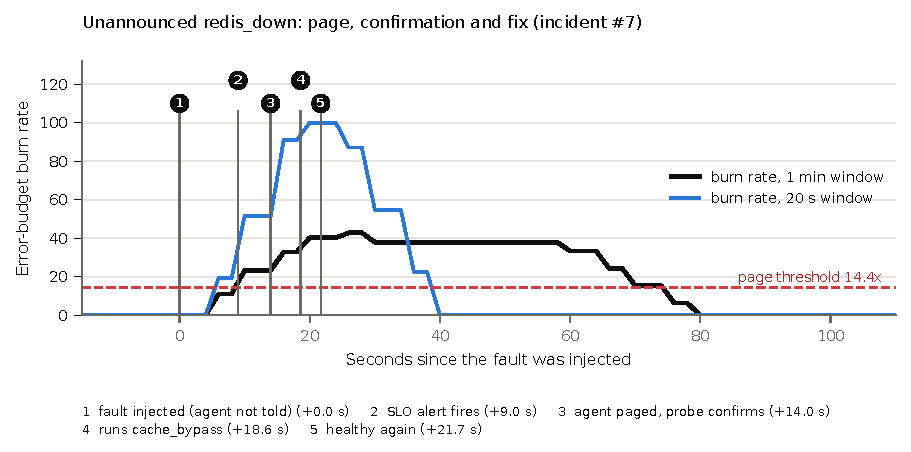
\includegraphics[width=0.92\textwidth]{fig_oncall_timeline.pdf}
\caption{An unannounced \act{redis\_down}, end to end. The 20\,s burn rate reacts first; the page
fires when the slower 1\,min window also exceeds 14.4 (multi-window rule). The agent confirms with
its own probe, runs \act{cache\_bypass}, and traffic is healthy about 24\,s after the fault; the alert
then clears as the windows drain.}
\label{fig:timeline}
\end{figure*}

\begin{table}[t]
\caption{On-call campaign: unannounced faults, three each, heuristic responder; medians in seconds
from injection to the alert, to the agent engaging, and to sustained healthy traffic.}
\label{tab:campaign}
\centering
\scriptsize
\setlength{\tabcolsep}{3pt}
\begin{tabular}{@{}lccccp{2.55cm}@{}}
\toprule
Failure & Healed & Alert & Engage & Healthy & Actions \\
\midrule
\texttt{redis\_down} & 3/3 & 10.2 & 14.7 & 21.7 & {\scriptsize cache\_bypass} \\
\texttt{redis\_latency} & 3/3 & 11.1 & 15.8 & 22.4 & {\scriptsize cache\_bypass} \\
\texttt{postgres\_latency} & 3/3 & 12.3 & 17.2 & 81.9 & {\scriptsize restart\_postgres,warm\_cache; warm\_cache} \\
\texttt{postgres\_down} & 3/3 & 14.5 & 19.0 & 34.7 & {\scriptsize restart\_postgres} \\
\texttt{api\_crash} & 3/3 & 12.8 & 17.4 & 36.3 & {\scriptsize restart\_api} \\
\midrule
\texttt{redis\_partition} & 3/3 & 11.5 & 16.1 & 21.0 & {\scriptsize cache\_bypass} \\
\texttt{redis\_down\_slow\_db} & 0/3 & 10.0 & 14.4 & -- & {\scriptsize cache\_bypass,restart\_postgres; cache\_bypass,restart\_postgres,restart\_redis} \\
\bottomrule
\end{tabular}
\end{table}

\begin{figure}[t]
\centering
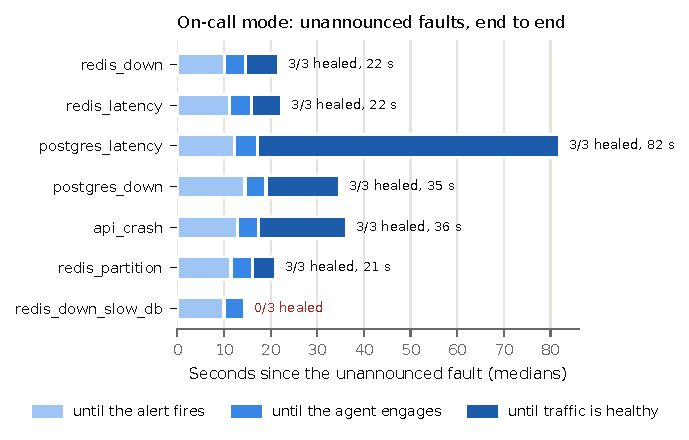
\includegraphics[width=\columnwidth]{fig_campaign.pdf}
\caption{On-call campaign, per fault: median time until the alert fires, the agent engages, and user
traffic is healthy again.}
\label{fig:campaign}
\end{figure}

Fig.~\ref{fig:timeline} traces one unannounced fault. Across the campaign
(Table~\ref{tab:campaign}, Fig.~\ref{fig:campaign}) the agent healed \ocHealed{} of \ocFaults{}
unannounced faults without being told what was injected. The median time from injection to the alert
was \ocMedDetect\,s, to the agent engaging \ocMedEngage\,s, and, for healed faults, to sustained healthy
traffic \ocMedRecover\,s; \ocEscalated{} incidents were escalated to a human, and \ocApprovals{}
high-impact actions ran only after the scripted operator's approval.
Detection was consistent across faults (10--15\,s to the alert, about 5\,s more until the agent was
paged and engaged), because it depends on the burn-rate windows rather than on the fault. Recovery
depended on the fix: about 21--22\,s for Redis faults healed by \act{cache\_bypass}, 35--36\,s for
crashed services that needed a restart (including the operator's 5\,s approval for
\act{restart\_postgres}). The slow database took longest (median 81.9\,s): pool timeouts made it look
unreachable, so the agent sometimes restarted PostgreSQL (with approval) before warming the cache,
the same ambiguity the bandit showed in experiments. All three compound faults were escalated after
the action budget was spent, and each escalation closed automatically once the lab was reset.

\begin{figure}[t]
\centering
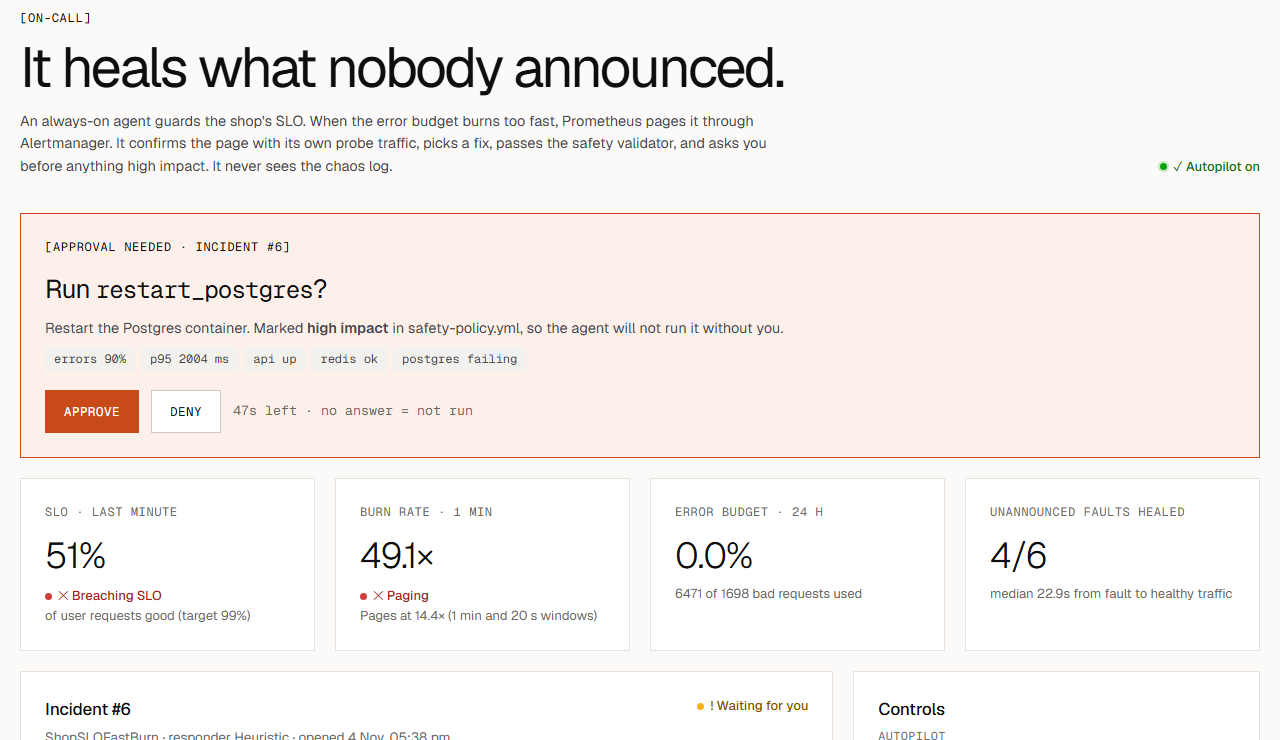
\includegraphics[width=\columnwidth]{screens/oncall-approval-crop.png}
\caption{The dashboard's on-call console during an unannounced \act{postgres\_down}: the agent proposes
the high-impact \act{restart\_postgres} and waits for a human decision; with no decision in 60\,s the
action is not run.}
\label{fig:approval}
\end{figure}

